\documentclass[11pt]{article}
\usepackage[T1]{fontenc}
\usepackage[utf8]{inputenc}
\usepackage{lmodern,amsmath,amssymb,graphicx,booktabs,array,microtype,xcolor}
\usepackage[margin=0.83in]{geometry}
\usepackage[colorlinks=true,linkcolor=teal,urlcolor=teal]{hyperref}
\setlength{\parindent}{0pt}
\setlength{\parskip}{6pt}
\setlength{\emergencystretch}{3em}
\title{\Huge Can one hear an aperiodic tile?\\[10pt]\large Spectral geometry, planar tiling and forced aperiodicity}
\author{A systematic research study prepared with Codex}
\date{7 October 2026}
\begin{document}
\maketitle


\textbf{Main finding.} An isolated tile's ordinary Laplacian eigenvalues are not currently a general certificate of forced aperiodicity. There are exact obstructions from missing placement rules, and a provable instability even for unmarked geometric monotiles. A much richer billiard invariant can recover many polygonal shapes; spectra of the entire tiling can detect long-range order under explicit assumptions.




\section*{1. Questions and study goals}


I chose five goals: define the spectral objects precisely; locate the strongest tiling theorems; distinguish impossibility results from unresolved inverse problems; investigate a family crossing between periodic tileability and forced aperiodicity; and identify what could become a useful certificate for tiling search. The literature study, analytic deductions and numerical experiment are completed here. The remaining questions are identified as research problems, not presented as solved.





\section*{2. Fix the object before asking the question}


A geometric tile is a bounded planar domain \(\Omega\) with a specified group \(G\) of allowed isometries. A tiling covers the plane with copies \(g_i\Omega\), with disjoint interiors. For measurable translational tilings, coverage and disjointness are understood almost everywhere. For marked tiles, matching rules are additional data.



A tiling \(\mathcal T\) has a translational period if \(\mathcal T+v=\mathcal T\) for a nonzero vector \(v\). A fully periodic tiling has two independent periods. In this study, a \textbf{strongly aperiodic tiling} has no nonzero translational period. A \textbf{forced-aperiodic tile} admits at least one tiling and every admitted tiling is strongly aperiodic. Merely constructing one nonperiodic arrangement does not establish this universal claim. Both the allowed group and the matching rules must be fixed.



\begin{center}\small
\setlength{\tabcolsep}{4pt}
\begin{tabular}{>{\raggedright\arraybackslash}p{0.2\linewidth}>{\raggedright\arraybackslash}p{0.34\linewidth}>{\raggedright\arraybackslash}p{0.38\linewidth}}
\toprule
\textbf{Data} & \textbf{What is measured?} & \textbf{Relationship to forced aperiodicity} \\
\midrule
Laplacian spectrum & Eigenvalues of an operator on the isolated tile, with chosen boundary conditions. & Geometric information and necessary inequalities; no general test established here. \\

Billiard length spectrum & Lengths of closed reflecting trajectories; marked versions retain trajectory labels. & Reflection geometry, with inverse results depending strongly on retained labels. \\

Bounce spectrum & The complete language of labeled boundary encounters. & Recovers non-right-angled polygons up to similarity; hence can determine geometric properties indirectly. \\

Fourier spectral set & An orthogonal basis of plane waves on the tile. & Equivalent to translational tileability for convex bodies; lattice cases certify a periodic option. \\

Diffraction spectrum & Fourier transform of the autocorrelation of a chosen decorated point pattern. & Detects long-range correlations of that pattern, with information loss. \\

Dynamical spectrum & Translation action on the space of legal tilings. & Can test periods if suitable eigenfunctions separate configurations. \\

\bottomrule
\end{tabular}
\end{center}


The first four start with a tile; the last two normally require a tiling or a tiling space. Confusing these levels would turn a statement about a known arrangement into an unsupported claim about every possible arrangement.




\section*{3. The strongest direct bridge: Fourier spectra}


A measurable domain is Fourier spectral if some countable frequency set \(\Lambda\) makes the normalized exponentials an orthonormal basis:


\[ e_\lambda(x)=|\Omega|^{-1/2}\exp(2\pi i\lambda\cdot x),\qquad \lambda\in\Lambda. \]

These are not generally Dirichlet or Neumann eigenfunctions on \(\Omega\). Their orthogonality means


\[ \widehat{\mathbf 1_\Omega}(\lambda-\mu)=0\quad(\lambda\ne\mu), \]

together with a completeness condition. Fuglede's conjecture linked this property to tiling by translations. For convex planar domains it is a theorem: spectrality is equivalent to translational tiling, and the tiles are parallelograms and centrally symmetric hexagons. Iosevich--Katz--Tao proved the planar result; Lev--Matolcsi later proved the convex-body equivalence in every dimension. \hyperlink{ref1}{[1]} \hyperlink{ref2}{[2]}



\subsection*{The lattice case has a transparent mechanism}


Let \(L\) be a full-rank lattice and \(L^*\) its reciprocal lattice. Periodize the indicator:


\[ P_L(x)=\sum_{\ell\in L}\mathbf 1_\Omega(x-\ell),\qquad L^*=\{k:k\cdot\ell\in\mathbb Z\text{ for every }\ell\in L\}. \]

Its Fourier coefficients are \(\widehat{\mathbf 1_\Omega}(k)/\operatorname{covol}(L)\). Therefore the exact conditions


\[ |\Omega|=\operatorname{covol}(L),\qquad \widehat{\mathbf 1_\Omega}(k)=0\quad(k\in L^*\setminus\{0\}) \]

are equivalent to \(P_L=1\) almost everywhere. They certify a lattice tiling and thus exclude forced aperiodicity for any allowed-placement model containing those translations. Testing finitely many Fourier zeros numerically does not certify this infinite set of conditions. A Fourier basis indexed by a reciprocal lattice supplies a periodic option; an arbitrary nonlattice Fourier spectrum does not automatically do so.



Every triangle can tile using appropriate congruent copies: a triangle and its half-turn make a parallelogram, which repeats. Yet a convex triangle is not Fourier spectral, by the planar classification. Thus ``not Fourier spectral'' does not imply ``cannot tile'' when rotations are permitted. \hyperlink{ref1}{[1]}



\textbf{Current literature status.} The unrestricted Fuglede equivalence fails in higher dimensions. A July 2026 preprint by Tao Zhang claims counterexamples to both directions already in the plane. I checked its statement and constructions at the source but have not independently validated its proof; this study does not rely on that claim. The established convex theorem and the lattice argument remain the relevant safe conclusions. \hyperlink{ref3}{[3]} \hyperlink{ref4}{[4]}




\section*{4. What the Laplacian does know about tiles}


For the Dirichlet drum, solve \(-\Delta u=\lambda u\) in \(\Omega\) with \(u|_{\partial\Omega}=0\); list eigenvalues \(0<\lambda_1\le\lambda_2\le\cdots\), including multiplicities. For Neumann conditions, \(\partial_\nu u=0\), the connected-domain spectrum begins \(0=\mu_0<\mu_1\le\cdots\). Scaling by \(s\) multiplies either spectrum by \(s^{-2}\); reflection and rotation leave it unchanged.



For a straight-sided polygon with interior angles \(\theta_i\), area \(A\) and perimeter \(P\), the Dirichlet heat trace has the expansion


\[ H_D(t)=\sum_{j\ge1}e^{-t\lambda_j}=\frac{A}{4\pi t}-\frac{P}{8\sqrt{\pi t}}+C_\Omega+O(e^{-c/t}),\qquad C_\Omega=\sum_i\frac{\pi^2-\theta_i^2}{24\pi\theta_i}. \]

Thus the spectrum determines these three geometric quantities. All further coefficients at algebraic orders vanish for such polygons; the full heat trace contains additional information beyond this expansion. In the class of triangles, area, perimeter and the reciprocal-angle sum determine the shape, giving a positive inverse spectral theorem. \hyperlink{ref5}{[5]}



For general planar domains, shape recovery fails: Gordon--Webb--Wolpert constructed noncongruent domains with identical full Dirichlet spectra. \textbf{That fact alone does not prove that tiling or aperiodicity differs within an isospectral pair.} Such a conclusion would require a pair with separately established, different tiling properties. I did not locate a verified geometric pair with one member forcing aperiodicity and the other admitting periodic tilings. \hyperlink{ref6}{[6]}



\subsection*{A genuine tiling-to-eigenvalues theorem}


Define \(N_D(E)=\#\{j:\lambda_j<E\}\) and \(N_N(E)=\#\{j:\mu_j<E\}\), including the Neumann zero mode. For planar tiling domains with the regularity needed for the operators, Pólya's inequalities give


\[ N_D(E)\le\frac{AE}{4\pi},\qquad N_N(E)\ge\frac{AE}{4\pi}\quad(E>0). \]

The mechanism is to fill a large region with copies of the tile and compare operators by boundary bracketing, then use Weyl asymptotics. Filonov supplies the general Neumann tiling result. The argument does not require that the chosen arrangement be periodic, so it cannot separate periodic tiles from forced-aperiodic ones. \hyperlink{ref7}{[7]}



The converse fails even as a tileability test: the disk obeys both inequalities but cannot tile the plane by congruent copies. A certified violation could reject tileability under the theorem's hypotheses; satisfying the inequalities does not establish it. \hyperlink{ref8}{[8]}




\section*{5. Geodesics, reflections and symbolic rigidity}


A flat domain's ordinary interior geodesics are straight lines. There is no useful collection of nonconstant closed interior geodesics. One must specify reflecting billiards, a doubled surface, or a surface formed by a prescribed edge gluing. Those last two constructions include data that the isolated tile does not supply on its own.



In a rectangle of side lengths \(a,b\), unfolding reflections gives closed-orbit lengths of the form \(2\sqrt{m^2a^2+n^2b^2}\), with admissible integer pairs and repetitions treated explicitly. Its Dirichlet spectrum is \(\pi^2(m^2/a^2+n^2/b^2)\) for positive integers. This common lattice geometry explains the relation in a special case; it is not a universal tiling criterion.



Rational polygon billiards unfold to compact translation surfaces, usually with cone singularities. The unfolded copies can overlap when projected to the plane. Compact unfolding therefore does not prove a plane tiling. Rational polygons include examples with quite different tiling behavior; rationality alone does not detect forced aperiodicity. \hyperlink{ref9}{[9]}



The wave trace \(\sum_j\cos(t\sqrt{\lambda_j})\), interpreted as a distribution, links eigenvalues to lengths of billiard trajectories. Corners introduce diffraction, and cancellations and degeneracies matter. One must not identify wave-trace singularities with a complete, labeled catalogue of all trajectories. Unmarked lengths discard which sides were encountered.



\textbf{A positive answer with richer data.} Duchin--Erlandsson--Leininger--Sadanand show that two simply connected Euclidean polygons with the same complete bounce spectrum are similar, except for the right-angled affine exception. The bounce spectrum records all bi-infinite sequences of side labels along nonsingular trajectories. For a non-right-angled polygon, it determines the shape up to similarity. With the placement rules fixed, the tiling and forced-aperiodicity properties are consequently determined as geometric properties of that recovered shape. This is an inference from their rigidity theorem, not a practical finite test or a theorem about unmarked lengths. \hyperlink{ref10}{[10]}



This applies to the polygonal Hat--Turtle family because its angles are not all multiples of \(\pi/2\). It does not extend directly to curved-edge Spectres. Recovering a shape also does not, by itself, provide a terminating algorithm to decide every tiling problem about that shape.




\section*{6. Three limits on detecting forced aperiodicity}


\subsection*{Placement rules are invisible to an ordinary drum}


The equilateral polygon \(\mathrm{Tile}(1,1)\) has periodic tilings if reflected copies are permitted. With reflections forbidden, its admitted tilings are all aperiodic. This is the weakly chiral monotile result. The physical domain and both its ordinary Dirichlet and Neumann spectra are identical in these two problems. Any detector using only those eigenvalues must give the same answer, even though the correct forced-aperiodicity answer changes. A detector must therefore accept the placement group as additional input. \hyperlink{ref11}{[11]}



\subsection*{Matching rules are also invisible unless coupled to the operator}


Adding arrows or colors to an unmodified tile boundary leaves a homogeneous drum unchanged. For example, the two Penrose rhombi with their matching rules force aperiodicity; without those rules each rhombus is a parallelogram admitting lattice tilings. The catalog of isolated shapes and its Laplacian spectra stay the same. This is an obstruction for decorated tile systems, not an isospectral counterexample between two different unmarked monotile shapes. \hyperlink{ref12}{[12]}



\subsection*{Even with fixed rules, finite noisy spectra are unstable}


Let \(\Omega_r=\mathrm{Tile}(1,r)\), with all planar isometries allowed. The established family result gives periodic tilings at \(r=1\), whereas every positive \(r\ne1\) forces aperiodicity. \hyperlink{ref13}{[13]} The boundary coordinates vary continuously. In a neighborhood of \(r=1\), a fixed triangulation gives a piecewise affine, bi-Lipschitz map from \(\Omega_1\) to \(\Omega_r\), tending to the identity.



\textit{Deduction in this study} Pull back the energy and mass forms through this map. Their Jacobians converge uniformly on the finitely many triangles. The min--max characterization then gives, for every fixed index \(j\),


\[ \lambda_j(\Omega_r)\longrightarrow\lambda_j(\Omega_1),\qquad \mu_j(\Omega_r)\longrightarrow\mu_j(\Omega_1)\quad(r\to1). \]

Area normalization preserves this convergence. Consequently, for any finite number \(K\) of modes and any positive measurement tolerance \(\varepsilon\), a forced-aperiodic member can satisfy


\[ \max_{1\le j\le K}\left|A_r\lambda_j(\Omega_r)-A_1\lambda_j(\Omega_1)\right|<\varepsilon. \]

The same statement holds for a finite combination of Dirichlet and Neumann modes. Their measurement intervals can overlap those of a periodically tileable member. Thus there is no universally robust finite-noise classifier over this family. This does \textbf{not} rule out a classifier using exact finite data in a restricted parametric family, or a decision theorem from the full exact infinite spectrum. Near equality is not isospectrality.




\section*{7. An exact counterexample for heat invariants}


\textit{Analytic deduction, not a full isospectral pair} There is a stronger failure for the usual heat invariants. For this family the angles are fixed, and direct geometry gives


\[ A(r)=\sqrt3(2+\sqrt3r+r^2),\qquad P(r)=8+6r,\qquad C(r)=\frac{11}{36}. \]

Choose a second ratio and scale it to the perimeter of the equilateral member:


\[ r_* =\frac{50\sqrt3-48}{22\sqrt3-27}\approx3.476103648,\qquad s_* =\frac{14}{8+6r_*}\approx0.485157273. \]

The equation \(P(r)^2/A(r)=P(1)^2/A(1)\) has exactly the roots \(1\) and \(r_*\). Indeed, after clearing the denominator it factors as


\[ (108-88\sqrt3)(r-1)(r-r_*)=0. \]

It follows that \(\Omega_1\) and \(s_*\Omega_{r_*}\) have exactly equal area, perimeter and corner heat constant. One admits periodic tilings; the other forces aperiodicity. Their \textbf{entire algebraic small-time Dirichlet heat expansions agree}, since a polygon has only the three nonzero coefficients displayed above. The exponentially small remainder and the full spectra need not agree.



This rules out forced-aperiodicity detection from those heat coefficients, even with exact measurements and a fixed group allowing all isometries. It illustrates why hearing corner complexity, or recovering a few global geometric invariants, is insufficient. The calculation is independently checked in the accompanying verification receipt.




\section*{8. A numerical investigation of the transition}


\begin{figure}[htbp]
\centering
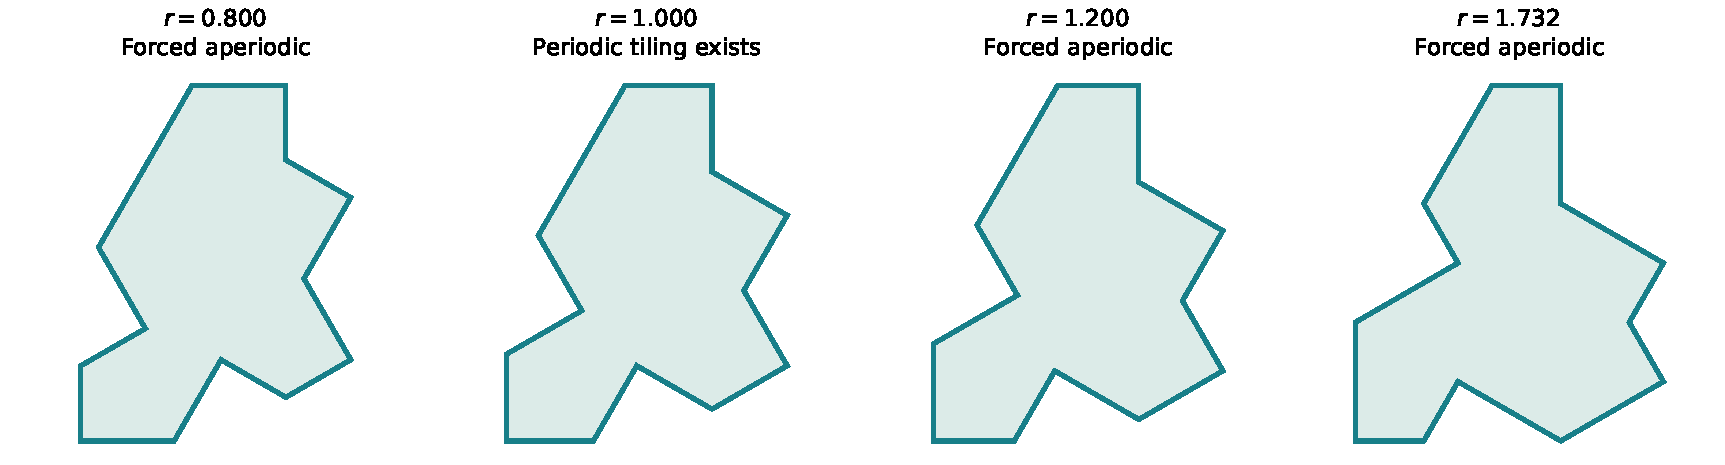
\includegraphics[width=\linewidth]{tile-family.pdf}

\caption{Shapes in the same geometric family. The labels are established by tiling theorems, not inferred from the eigenvalues. All isometries, including reflections, are allowed.}

\end{figure}


The computation estimates the first twelve Dirichlet eigenvalues at ten parameter values. It uses conforming linear finite elements, a consistent mass matrix, a constrained quality triangulation, a common deformation of that mesh, and three nested refinements. The reported feature is \(A_r\lambda_j\), which removes overall scale. The same isolated tile, without an added potential or matching-rule boundary condition, is used throughout.



\begin{figure}[htbp]
\centering
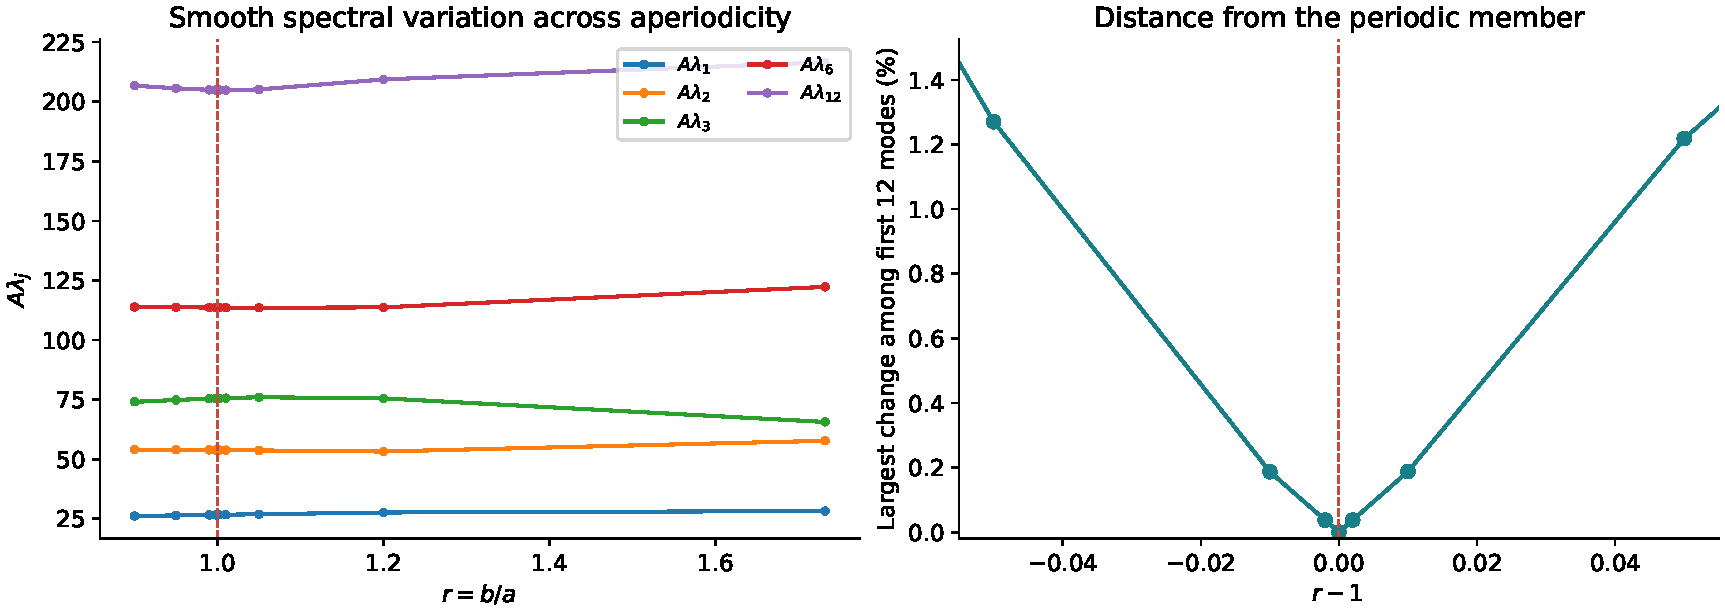
\includegraphics[width=\linewidth]{spectral-continuity.pdf}

\caption{The red line marks the equilateral parameter, where periodic tilings are possible. Nearby parameter values force aperiodicity. The smooth numerical variation illustrates the min--max continuity deduction; it is not its proof.}

\end{figure}


\begin{center}\small
\setlength{\tabcolsep}{4pt}
\begin{tabular}{>{\raggedright\arraybackslash}p{0.2\linewidth}>{\raggedright\arraybackslash}p{0.34\linewidth}>{\raggedright\arraybackslash}p{0.38\linewidth}}
\toprule
\textbf{Ratio} & \textbf{Known tiling property} & \textbf{Largest relative change in first twelve modes} \\
\midrule
\(0.9\) & forces aperiodicity & \(3.092\%\) \\

\(0.95\) & forces aperiodicity & \(1.271\%\) \\

\(0.99\) & forces aperiodicity & \(0.1871\%\) \\

\(0.998\) & forces aperiodicity & \(0.0375\%\) \\

\(1\) & admits periodic tilings & \(0\%\) \\

\(1.002\) & forces aperiodicity & \(0.03753\%\) \\

\(1.01\) & forces aperiodicity & \(0.188\%\) \\

\(1.05\) & forces aperiodicity & \(1.219\%\) \\

\(1.2\) & forces aperiodicity & \(4.045\%\) \\

\(1.73205\) & forces aperiodicity & \(13.11\%\) \\

\bottomrule
\end{tabular}
\end{center}


Each finest family mesh has \(17065\) nodes and \(33664\) triangles. The largest last-refinement change among the twelve modes is \(1.231\%\) over all cases, and \(0.409\%\) for \(0.95\le r\le1.05\). The finest square control differs from its exact first twelve modes by at most \(0.106\%\). The largest reported relative eigensolver residual is \(2.86\times10^{-11}\).



Refinement differences measure sensitivity to discretization; they are not rigorous error bounds. A tiny algebraic eigensolver residual is also not a bound on the continuum eigenvalue error. Common meshes help isolate the variation with the parameter, but do not eliminate discretization error. In particular, the small spectral differences near the equilateral member are numerical illustrations, while the analytic continuity argument establishes arbitrary closeness independently.



The experiment has no trained classifier and no inference of labels from a finite patch. It does not claim to discover a new monotile or to independently reprove the Hat-family aperiodicity theorem.




\section*{9. Where aperiodicity really appears spectrally}


\subsection*{Diffraction combines a tile with its arrangement}


For translates in a finite patch, the Fourier amplitude of a density formed by copies of the tile factors as


\[ \widehat\rho(k)=\widehat{\mathbf 1_\Omega}(k)\sum_{x\in\Lambda}e^{-2\pi i k\cdot x}. \]

The first factor is the tile's form factor; the second depends on the arrangement of copies. Rotated tiles require separate orientation contributions. Exact tiling by uniform density has \(\rho=1\) almost everywhere, so it produces only the trivial zero-frequency contribution: \textbf{an observation that erases tile boundaries can erase all aperiodicity information.} Useful diffraction needs control points, vertex sets, boundary contrast or another specified decoration.



For a suitable translation-bounded point measure \(\omega\), its autocorrelation is the volume-averaged convolution \(\gamma\), and its diffraction is \(\widehat\gamma\). Sharp Bragg peaks do not imply periodicity. Hat-family tiling dynamics have pure point spectrum, and the diffraction of Hat and Spectre tilings has now been derived through model-set representatives and reprojections. These are spectral results about their long-range tilings, not the isolated drum. \hyperlink{ref14}{[14]} \hyperlink{ref15}{[15]}



A periodic decorated pattern has diffraction supported on a reciprocal lattice. Incommensurate nonzero peaks can exclude candidate period lattices; a finite diffraction image usually cannot certify exact incommensurability. Extinctions may hide relevant frequencies. Distinct homometric structures share autocorrelation and diffraction, so diffraction generally does not reconstruct all boundary or matching information. \hyperlink{ref16}{[16]}



\subsection*{Dynamical eigenfunctions test translation periods}


Let \(X\) be a specified legal tiling space. A continuous translation eigenfunction obeys


\[ f_k(T-v)=e^{2\pi i k\cdot v}f_k(T). \]

If \(v\) is a period of \(T\) and \(f_k(T)\ne0\), then \(k\cdot v\in\mathbb Z\). Thus available eigenfrequencies constrain its periods through


\[ \operatorname{Per}(T)\subseteq\{v:k\cdot v\in\mathbb Z\text{ for all such }k\}. \]

\textit{Conditional certificate} If this annihilator is trivial, those eigenfunctions certify that the configuration has no nonzero period. If continuous eigenfunctions separate configurations and the condition applies throughout the full legal space, it can certify forced aperiodicity of that space. Measure-theoretic statements about almost every tiling alone do not exclude exceptional periodic tilings. Counting the rank of the frequency module alone also need not exclude a remaining one-dimensional period.



Pure point diffraction and pure point dynamical spectrum are equivalent in the appropriate finite-local-complexity setting with uniform cluster frequencies, retaining the relevant colors or observables. A single observation can lose information. \hyperlink{ref17}{[17]} Before this helps the monotile question, one must establish that the studied space includes every legal tiling of that tile.



\subsection*{A Laplacian on the full tiled plane needs an interface model}


If all seams are transparent and the operator is simply the Euclidean Laplacian on the whole plane, its spectrum is \([0,\infty)\), regardless of the tiling. If each tile is isolated by Dirichlet walls, the direct-sum spectrum repeats the same tile eigenvalues and forgets its arrangement. Geometry can influence an operator with seam interactions, graph adjacency, varying material coefficients or a tiling-dependent potential, but those are additional models. Band gaps, localized states and level statistics are then model-dependent observations, not automatic certificates of forced aperiodicity.




\section*{10. What I would investigate next}


The evidence favors \textbf{boundary and compatibility information} over a scalar eigenvalue fingerprint. The following priorities each have a concrete success criterion.



\begin{enumerate}


\item \textbf{Resolve the exact-spectrum question with fixed placement rules.} Seek either an isospectral pair of unmarked planar monotiles with different forced-aperiodicity status, or an inverse theorem for a meaningful class containing known monotiles. A pair must have a certified infinite construction for each tiler and a proof excluding every periodic tiling for the aperiodic member. Noncongruence alone is insufficient. This study establishes no such pair.

\item \textbf{Study boundary response and attachment.} Retain a parameterized Dirichlet-to-Neumann operator or boundary eigenfunction data, rather than just eigenvalues. Gluing two boundaries needs continuity of the field and cancellation of outward flux, information scalar spectra omit. Inverse boundary spectral results exist under precise admissibility assumptions; they are a reason to study richer data, not a blanket reconstruction theorem for every tile. \hyperlink{ref18}{[18]} Success would be an exact reduction of some boundary incompatibility to an independently checkable spectral certificate.

\item \textbf{Exploit complete bounce data in polygonal families.} Use symbolic rigidity to recover geometry in the non-right-angled class, then apply geometric tiling theorems. The target is a restricted reconstruction procedure with a declared completeness guarantee. A finite collection of sampled trajectories must not be treated as the complete bounce language.

\item \textbf{Build a full-space dynamical certificate.} Identify a forced hierarchy for every legal tiling, derive its translation eigenfunctions, and show their period annihilator is trivial. A substitution generating some aperiodic examples is insufficient; recognition and exhaustive coverage of legal configurations are the decisive steps.

\end{enumerate}


In a known parametric family such as \(\mathrm{Tile}(1,r)\), exact geometry already supplies the aperiodicity answer. Spectral measurements could estimate the parameter and thereby suggest a label, but the guarantee would come from the family theorem. It would not transfer automatically to arbitrary custom tiles.




\section*{11. Implications for GCTS and proof scope}


This study changes no tiling engine. Its finite-element solver is a continuum spectral experiment, not an implementation of the point-value tiling baseline. I read the project's master algorithm contract; no conformance to its frontier scheduler or candidate graph is claimed for the FEM computation.



For future integration, spectral features may rank candidates within the permitted generation ties or help propose clusters. They must not silently remove candidates. A proved Fourier lattice identity can certify a periodic construction; a proved necessary spectral inequality may justify an exclusion under its hypotheses. A learned spectral correlation remains a hypothesis and cannot turn budget exhaustion into non-tiling or forced aperiodicity.



The base tiling model must still specify the exact point domain, values, markings and allowed transforms; maintain complete point--candidate incidence; check global dead ends and forced moves before earliest-generation branching; preserve exact rollback; and independently verify all occupancy and matching claims. The continuum-to-point reduction itself needs justification. A spectral score does not replace those obligations.




\section*{12. Answers to the original questions}


\begin{itemize}


\item \textbf{Can spectra connect to whether a tile tiles?} Yes: Fourier spectrality characterizes convex translational tiles; lattice Fourier conditions certify periodic constructions; Laplacian inequalities are necessary for tiling domains.

\item \textbf{Can ordinary drum data determine forced aperiodicity?} The answer is no if placement rules or decorations are omitted. Exact heat coefficients fail even with fixed rules. Finite noisy modes have a provable instability. For the full exact infinite Laplacian spectrum of an unmarked geometric tile with rules fixed, this study leaves the general question unresolved.

\item \textbf{Can geodesic information help?} Complete symbolic billiard data can determine non-right-angled polygons up to similarity, so it determines their geometric tiling properties indirectly. Ordinary unmarked lengths are a different, weaker input.

\item \textbf{Which spectrum is most relevant to aperiodic order?} The translation dynamics of the complete legal tiling space, supported by specified diffraction observables, has the strongest direct relationship. It still needs a theorem connecting that space to every allowed tiling of the tile.

\end{itemize}



\section*{Primary sources and audit trail}


Sources checked on 7 October 2026. Established theorems, a recent preprint claim, deductions in this study and numerical observations are distinguished in the text. The search focused on Fourier tiling, inverse planar spectra, billiard rigidity and Hat/Spectre dynamics; this is a systematic thematic study, not an exhaustive bibliometric review.



\begin{enumerate}


\item \hypertarget{ref1}{}Iosevich, Katz and Tao. \href{https://arxiv.org/abs/math/0104087}{Fuglede conjecture holds for convex planar domains}. Mathematical Research Letters, 2003. Planar convex equivalence and classification.

\item \hypertarget{ref2}{}Lev and Matolcsi. \href{https://arxiv.org/abs/1904.12262}{The Fuglede conjecture for convex domains is true in all dimensions}. Convex-body theorem.

\item \hypertarget{ref3}{}Kolountzakis. \href{https://arxiv.org/abs/2509.05782}{Fuglede's conjecture on orthogonal bases of exponentials}, 2025. Context on the original spectral-set problem.

\item \hypertarget{ref4}{}Tao Zhang. \href{https://arxiv.org/abs/2607.15632}{Both directions of Fuglede's conjecture fail in dimension two}, July 2026, preprint. Recent claim; not independently validated here.

\item \hypertarget{ref5}{}Grieser and Maronna. \href{https://arxiv.org/abs/1208.3163}{Hearing the shape of a triangle}. Polygon heat trace and triangular rigidity.

\item \hypertarget{ref6}{}Gordon, Webb and Wolpert. \href{https://arxiv.org/abs/math/9207215}{One cannot hear the shape of a drum}, 1992. Planar isospectral noncongruence.

\item \hypertarget{ref7}{}Filonov. \href{https://arxiv.org/abs/2006.10663}{On the Pólya conjecture for the Neumann problem in tiling sets}, 2020. Neumann tiling inequality.

\item \hypertarget{ref8}{}Filonov, Levitin, Polterovich and Sher. \href{https://arxiv.org/abs/2203.07696}{Pólya's conjecture for Euclidean balls}. Inventiones Mathematicae, 2023. Disk counterexample to a tiling converse.

\item \hypertarget{ref9}{}Masur and Tabachnikov. \href{https://math.uchicago.edu/~masur/handbook1.pdf}{Rational billiards and flat structures}. Unfolding and translation surfaces.

\item \hypertarget{ref10}{}Duchin, Erlandsson, Leininger and Sadanand. \href{https://arxiv.org/abs/1804.05690}{You can hear the shape of a billiard table: Symbolic dynamics and rigidity for flat surfaces}. Commentarii Mathematici Helvetici, 2021. Bounce rigidity theorem.

\item \hypertarget{ref11}{}Smith, Myers, Kaplan and Goodman-Strauss. \href{https://arxiv.org/abs/2305.17743}{A chiral aperiodic monotile}. Equilateral weak chirality and Spectre construction.

\item \hypertarget{ref12}{}de Bruijn. \href{https://doi.org/10.1016/1385-7258(81)90016-0}{Algebraic theory of Penrose's non-periodic tilings of the plane. I}. Indagationes Mathematicae, 1981. Penrose tilings and matching rules.

\item \hypertarget{ref13}{}Smith, Myers, Kaplan and Goodman-Strauss. \href{https://arxiv.org/abs/2303.10798}{An aperiodic monotile}. Combinatorial Theory, 2024; especially Section 6 for the parameter family.

\item \hypertarget{ref14}{}Baake, Gähler and Sadun. \href{https://arxiv.org/abs/2305.05639}{Dynamics and topology of the Hat family of tilings}. Israel Journal of Mathematics, 2025. CAP model sets and Hat dynamics.

\item \hypertarget{ref15}{}Baake, Gähler, Mazáč and Mitchell. \href{https://arxiv.org/abs/2502.03268}{Diffraction of the Hat and Spectre tilings and some of their relatives}. Explicit diffraction via model sets and reprojection.

\item \hypertarget{ref16}{}Baake and Grimm. \href{https://arxiv.org/abs/math/0610411}{Homometric model sets and window covariograms}. Nonuniqueness of diffraction reconstruction.

\item \hypertarget{ref17}{}Lee, Moody and Solomyak. \href{https://arxiv.org/abs/0910.4809}{Pure Point Dynamical and Diffraction Spectra}. Equivalence under stated local-complexity and frequency hypotheses.

\item \hypertarget{ref18}{}Kirpichnikova and Kurylev. \href{https://arxiv.org/abs/math/0701911}{Inverse boundary spectral problem for Riemannian polyhedra}. Boundary data uniqueness with admissibility assumptions.

\end{enumerate}


Additional verified context: \href{https://arxiv.org/abs/1602.05738}{Bhattacharya's planar lattice translational periodicity theorem} says a finite subset of the integer plane that tiles by translations has a fully periodic tiling. It concerns that lattice model, not arbitrary rotations of a Euclidean monotile.



\end{document}
